\section{Iconix}

\par O ICONIX, segundo \citeonline{rosenberg_iconix_process}, foi criado em 1993 a partir de um resumo das melhores técnicas de desenvolvimento de \textit{software} utilizando como ferramenta de apoio a \textit{Unified Modeling Language} - UML\footnotemark[3]. Esta metodologia é mantida pela empresa ICONIX \textit{Software Engineering} e seu principal idealizador é Doug Rosenberg.

%Nota a respeito da sigla UML
\footnotetext[3]{UML: \textit{Unified Modeling Language} - Linguagem de modelagem para objetos do mundo real que habilita os desenvolvedores especificar, visualizar, construí-los a nível de software.}


\par Para \citeonline{rosenberg_scott_use_case_driven_object_modeling_with_uml}, o ICONIX possui como característica ser iterativo e incremental, somado ao fato de ser adequado ao padrão UML auxiliando, assim, o desenvolvimento e a documentação do sistema.

\par Atualmente, existem diversas metodologias de desenvolvimento de \textit{software} disponíveis, contudo, o ICONIX, em especial, será utilizado para auxiliar no processo de desenvolvimento deste trabalho pois, segundo
\citeonline{silva_videira_uml_metodologias_ferramentas_case}, esta metodologia nos permite gerar a documentação necessária para nortear o desenvolvimento de um projeto acadêmico.

\par De acordo com \citeonline{rosenberg_stephens_use_case_driven_object_modeling_with_uml}, os processos do ICONIX consistem em gerar alguns artefatos que correspondem aos modelos dinâmico e estático de um sistema e estes são elaborados e desenvolvidos de forma incremental e em paralelo, possibilitando ao analista dar maior ênfase no desenvolvimento do sistema do que na documentação do mesmo. A figura 1, apresenta uma visão geral dos componentes do ICONIX.

% Imagem do Iconix
\begin{figure}[h!]
	\centerline{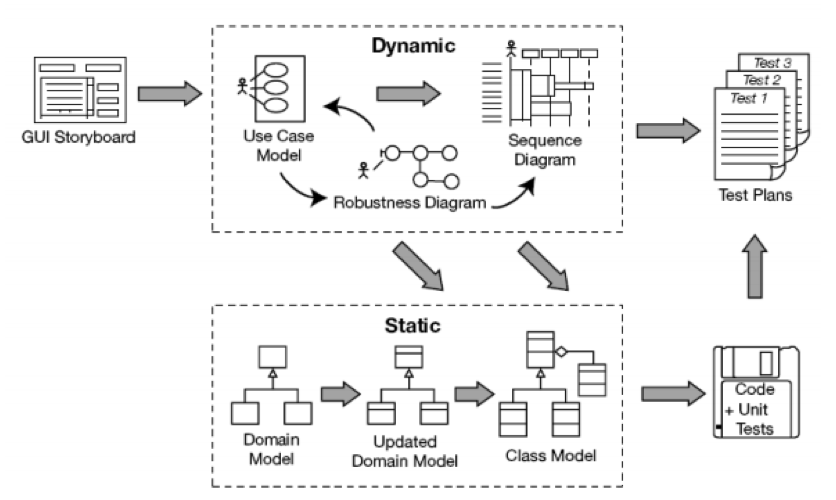
\includegraphics[scale=0.95]{./imagens/visao_geral_iconix.png}}
	\caption[Uma visão geral do ICONIX e seus componentes.]
	{Uma visão geral do ICONIX e seus componentes. \textbf{Fonte:} \citeonline{rosenberg_scott_use_case_driven_object_modeling_with_uml}}
	\label{fig:exemplo1}
\end{figure}

\newpage %Pular pagina para que o texto fica abaixo da imagem na nova pagina

\par Ao utilizar esta metodologia, o desenvolvimento do projeto passa a ser norteado por casos de uso(\textit{use cases}) e suas principais fases são: análise de requisitos, análise e projeto preliminar, projeto e implementação. Abaixo será apresentado uma breve descrição de cada uma das fases do ICONIX, seguindo ideias de \citeonline{o_engenheiro_software_as_fases_iconix_mecva}.

\subsection{Análise de requisitos}

Identificar os objetos do problema real e como eles serão abstraídos para um objeto de software através dos modelos de domínio; apresentar um protótipo das possíveis interfaces gráficas, e por fim descrever os casos de uso. 

Se possível, elaborar também os diagramas de navegação para que o cliente possa entender melhor o funcionamento do sistema como um todo.

\subsection{Análise e projeto preliminar}

Detalhar todos os casos de uso identificados na fase de requisitos, por meio de diagramas de robustez, baseando-se no texto dos casos de uso (fluxo de eventos). O diagrama de robustez não faz parte dos diagramas padrões da UML. Porém, este é utilizado para descobrir as classes de análise e detalhar superficialmente o funcionamento dos casos de uso.

Em paralelo, deve-se atualizar o modelo de domínio adicionando os atributos às entidades identificados. A partir deste momento será possível gerar a base de dados do sistema.


\subsection{Projeto detalhado}

Elaborar o diagrama de sequência fundamentando-se nos diagramas de casos de uso identificados anteriormente, a fim de detalhar a implementação do caso de uso.

O diagrama de sequência deve conter as classes que serão implementadas e as mensagens enviadas entre os objetos, corresponderão aos métodos que realmente serão implementados futuramente.
 

\subsection{Implementação}

Desenvolver o código fonte e os testes do sistema. O ICONIX não define os passos a serem seguidos nesta fase, ficando a cargo da equipe de desenvolvimento.
 
Ao término de cada fase um artefato é gerado, sendo respectivamente: revisão dos requisitos, revisão do projeto preliminar, revisão detalhada e entrega.

O ICONIX é considerado um processo prático de desenvolvimento de software, pois a partir das iterações que ocorrem na análise de requisitos e na construção dos modelos de domínios (parte dinâmica), os diagramas de classes (parte estática) são incrementados e a partir destes, o sistema poderá ser codificado.


Por proporcionar esta praticidade, o ICONIX será empregado para o desenvolvimento deste projeto, pois por meio dele é possível obter produtividade no desenvolvimento do \textit{software} ao mesmo tempo em que alguns artefatos são gerados, unindo o aspecto de abrangência e agilidade.
